\chapter{IMPLEMENTASI}
Setelah melewati proses perancangan mengenai sistem yang akan dibuat, maka akan dilakukan implementasi dari sistem tersebut. Bab ini akan membahas mengenai implementasi dari sistem yang meliputi proses pembuatan setiap komponen sehingga sistem dapat berjalan dengan baik. Masing-proses pembuat komponen akan dilengkapi dengan \textit{pseudocode} atau konfigurasi dari sistem.  
\section{Lingkungan Implementasi}
  	Dalam mengimplementasikan sistem, digunakan beberapa perangkat pendukung sebagai ebrikut.
    \subsection{Perangkat Keras}
    Perangkat keras yang digunakan dalam pengembangan sistem adalah sebagai berikut:
    \begin{enumerate}
    \item Komputer dengan \textit{processor} Intel(R) Core(TM) i5-2120 CPU @ 3.30GHz dan RAM 8GB
    \item Dua Komputer dengan \textit{processor} Intel(R) Core(TM)2 Duo CPU E7200 @ 2.53GHz dan RAM 1GB
    \end{enumerate}
    \subsection{Perangkat Lunak}
    Perangkat lunak yang digunakan dalam pengembangan sistem adalah sebagai berikut:
    \begin{enumerate}
    \item Sistem Operasi Linux Mint 18.03 64 Bit sebagai \textit{docker host}.
    \item Sistem Operasi Ubuntu 14.04 LTS 64 Bit sebagai \textit{client}.
    \item \textit{Python} versi 3.5.2 untuk pengembangan web service. 
    \item \textit{Flask} versi 1.0.2 sebagai Kerangka Kerja \textit{Python}.
    \item \textit{Gunicorn} versi 19.8.1
    \item \textit{Supervisor} versi 3.2.0
    \item \textit{Nginx} versi
    \item \textit{Mitmproxy} versi 3.0.4 untuk mencatat semua \textit{traffic} dari \textit{client}.
    \item MySQL versi 5.7.18 untuk Sistem Manajemen Basis Data.
    \item \textit{Docker} versi 1.13.1 sebagai kontainer yang akan di pasangkan pada \textit{server}.
    \item \textit{Iptables} versi 1.6.0 untuk membuat aturan terhadap \textit{client}.
    \item \textit{VIM} versi 7.4.1 sebagai \textit{text editor}.
    \end{enumerate}
  
  \section{Implementasi Pembuatan Aturan untuk Mengarahkan \textit{Traffic Client} ke Halaman \textit{Login} dari Sistem}
  Pada implementasi pembuatan aturan untuk mengarahkan \textit{traffic client} ke halaman \textit{Login} dari sistem diasumsikan bahwa belum ada \textit{client} yang telah \textit{login} ke dalam sistem. Lalu dibuatkan beberapa \textit{rules} dengan menggunakan \textit{iptables} seperti Kode Sumber \ref{iptablesbeforelogin}. \\
  \begin{minipage}{\linewidth}
  	\begin{lstlisting}[caption=Command untuk mengarahkan \textit{client} ke halaman \textit{login},language=Python,label=iptablesbeforelogin]
  	iptables -I FORWARD 1 -s 192.168.99.0/24 -j REJECT
  	iptables -I FORWARD 1 -s 192.168.99.0/24 -p tcp d 10.151.36.130
  	--dport 4000 -j ACCEPT
  	iptables -t nat -I PREROUTING 1 -p tcp -s 192.168.99.0/24
  	--dport 80 -j DNAT --to 10.151.36.130:4000
  	\end{lstlisting}
  \end{minipage}
  
  \textit{Rules} pertama berfungsi untuk tidak memperbolehkan semua \textit{client} untuk melewati \textit{router}. Lalu \textit{rules} kedua berfungsi untuk memperbolehkan semua \textit{client} untuk membuka halaman \textit{login}. Lalu \textit{rules} ketiga berfungsi untuk mengarahkan semua \textit{traffic client} ke halaman \textit{login}. Pada gambar \ref{diagram2} ditunjukkan arsitektur sistem saat \textit{traffic} dari salah satu \textit{client} diarahkan ke halaman \textit{login} dari sebuah sistem.
  
  \begin{figure}[H]
  	\centering
  	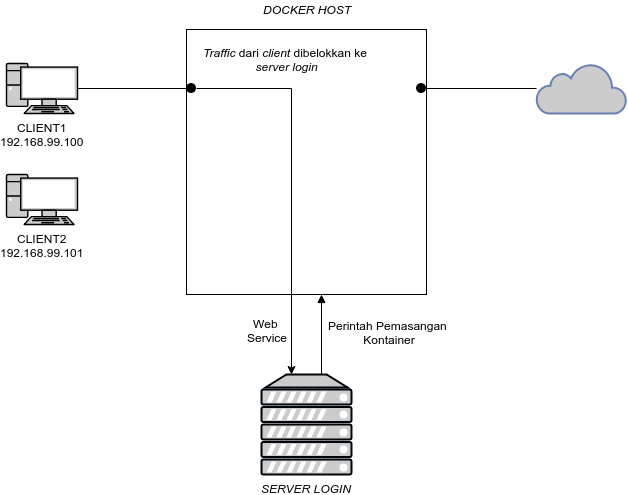
\includegraphics[width=\linewidth]{images/bab4/DIAGRAM2}
  	\caption{Arsitektur saat \textit{Traffic} dari \textit{Client} Diarahkan ke Halaman \textit{Login}}
  	\label{diagram2}
  \end{figure} 
  
  \section{Implementasi Pembuatan Halaman \textit{Login}}
  Pada implementasi pembuatan halaman \textit{login}, dibutuhkan beberapa persiapan lingkungan implementasi yang perlu dilakukan, meliputi langkah-langkah berikut:
  \begin{enumerate}
  	\item Instalasi \textit{Python} versi 3.5.2
  	\item Instalasi \textit{Flask} versi 1.0.2
  \end{enumerate}
  \textit{Python} akan berfungsi sebagai komponen dasar pembangunan sistem, salah satunya adalah sebagai komponen dasar pembuatan halaman \textit{login}, sedangkan \textit{Flask} akan berfungsi sebagai kerangka kerja untuk pembuatan halaman \textit{lgin}. Untuk melakukan pemasangan \textit{Python} versi 3.5.2 pada sistem operasi Ubuntu, lalu jalankan \textit{command} pada terminal seperti Kode Sumber \ref{installpython3}.\\
  \begin{minipage}{\linewidth}
  	\begin{lstlisting}[caption=Command untuk installasi Python,language=Python,label=installpython3]
  	sudo apt-get update
  	sudo apt-get install python3
  	\end{lstlisting}
  \end{minipage}
  Lalu, untuk melakukan pemasangan \textit{Flask} versi 1.0.2 pada sistem operasi ubuntu jalankan \textit{command} pada terminal seperti Kode Sumber \ref{installflask}.\\
	\begin{minipage}{\linewidth}
	   	\begin{lstlisting}[caption=Command untuk installasi Flask,language=Python,label=installflask]
	   	sudo apt-get install python3-pip
	   	sudo pip install flask
	   	\end{lstlisting}
	\end{minipage}
	
  \section{Implementasi \textit{Middleware}}
  \textit{Middleware} merupakan komponen yang akan menerima permintaan dari \textit{client}, mengirimkan perintah untuk membuat kontainer \textit{docker} secara otomatis pada \textit{docker host}, dan menentukan rute \textit{traffic} dari \textit{client} menuju ke internet sesuai kontainer \textit{docker} masing-masing user. Implementasi \textit{middleware} akan terbagi menjadi implementasi basis data dan implementasi \textit{web service}.
  \subsection{Implementasi Basis Data}
  Berdasarkan hasil perancangan basis data pada bab 3 terdapat 2 entitas yang diimplementasikan menjadi suatu tabel pada basis data MySQL, yaitu entitas \textit{testing} dan entitas nrp-mahasiswa. Detail implementasi entitas \textit{testing} tertera pada Kode Sumber \ref{entitastesting}.
  \newline
  \begin{minipage}{\linewidth}
  	\begin{lstlisting}[language=python, caption=\textit{Query} untuk membuat tabel testing,label=entitastesting]
  	CREATE TABLE testing (
	  	id int(11) PRIMARY KEY AUTO_INCREMENT,
	  	username VARCHAR(50)
	  	ip VARCHAR(50)
	  	createdAt DATETIME
  	);
  	\end{lstlisting}
  \end{minipage}
  Sedangkan untuk detail implementasi entitas nrp-mahasiswa tertera pada Kode Sumber \ref{entitasnrpmahasiswa}.
    \newline
    \begin{minipage}{\linewidth}
    \begin{lstlisting}[language=python, caption=\textit{Query} untuk membuat tabel testing,label=entitasnrpmahasiswa]
    CREATE TABLE nrp-mahasiswa (
    	id int(11) PRIMARY KEY AUTO_INCREMENT,
    	nrp VARCHAR(50)
    	password VARCHAR(50)
    	isLogin int(11)
    );
    \end{lstlisting}
    \end{minipage}
    
  \subsection{Implementasi \textit{Web Service}}
  Pada implementasi \textit{web service} dibutuhkan beberapa persiapan lingkungan implementasi yang perlu dilakukan, meliputi langkah-langkah berikut:
    \begin{enumerate}
    	\item Instalasi \textit{Python} versi 3.5.2
    	\item Instalasi \textit{Flask} versi 1.0.2
    \end{enumerate}
  \textit{Python} akan berfungsi sebagai komponen dasar pembangunan sistem, salah satunya adalah sebagai komponen dasar pembuatan \textit{middleware}, sedangkan \textit{Flask} akan berfungsi sebagai kerangka kerja untuk pembuatan \textit{middleware}.
  \subsubsection{Rute \textit{Web Service}}
  \textit{Middleware} tidak memiliki antar muka grafis. Namun diperlukan adanya rute-rute yang bisa diakses untuk melayani permintaan penyediaan kontainer \textit{docker} dari \textit{client}. Daftar rute yang disediakan oleh \textit{middleware} tertera pada Tabel \ref{tabelRuteWebService}
  \begin{longtable}{|p{0.15\textwidth}|p{0.25\textwidth}|p{0.3\textwidth}|p{0.3\textwidth}|} % L = Rata kiri untuk setiap kolom, | = garis batas vertikal.
  	
  	% Kepala tabel, berulang di setiap halaman
  	\caption{Daftar Rute \textit{Web Service}} \label{tabelRuteWebService} \\
  	\hline
  	\textbf{HTTP Method} & \textbf{Rute} & \textbf{Deskripsi} \\ \hline
  	
  	\endfirsthead
  	\caption[]{Daftar Rute \textit{Web Service}}  \\
  	\hline
  	\textbf{HTTP Method} & \textbf{Rute} & \textbf{Deskripsi}  \\ \hline
  	
  	\endhead
  	\endfoot
  	\endlastfoot
  	
  	% Isi Tabel
  	POST & /test/endpoint/ & Berfungsi untuk menyimpan data hasil \textit{input} dari \textit{client} dan mengirimkan perintah untuk membuat kontainer \textit{docker} yang berisikan \textit{mitmproxy} secara otomatis pada \textit{docker host}.\\ \hline
  \end{longtable}
  
  \subsection{\textit{Pseduocode Web Service}}
  Saat \textit{client} telah memasukkan \textit{input} ke sistem, sistem akan mencocokkan terlebih dahulu dengan basis data nrp-mahasiswa. Jika benar, maka sistem akan mengirimkan data \textit{input} dari \textit{client} ke \textit{middleware}. Lalu \textit{middleware} akan menyimpan data \textit{input} dari \textit{client} ke dalam sebuah \textit{file}. Setelah itu \textit{middleware} akan mengirimkan perintah untuk membuat sebuah kontainer \textit{docker} yang berisikan \textit{mitmproxy} pada \textit{docker host}.
  
  Saat \textit{middleware} menyimpan data \textit{input} dari \textit{client} ke dalam sebuah \textit{file}, yang disimpan adalah \textit{username} atau NRP, \textit{IP Address}, dan \textit{port}. Nantinya \textit{port} tersebut akan menjadi \textit{port} khusus untuk kontainer \textit{docker} yang berisikan \textit{mitmproxy} untuk \textit{client} tersebut.
  
  Saat kontainer \textit{docker} yang berisikan \textit{mitmproxy} akan dibuat pada \textit{docker host}, sistem akan membuat kontainer \textit{docker} dengan \textit{mode network}=\textit{host}, nama sesuai \textit{IP Address} dari \textit{client} tersebut, dan \textit{port} kontainer \textit{docker} sesuai dengan \textit{port} yang sudah disimpan pada \textit{file}.
  
  Setelah kontainer \textit{docker} yang berisikan \textit{mitmproxy} berhasil dibuat, maka sistem akan membuat \textit{rules} yang berfungsi untuk mengarahkan traffic dari \textit{client} menuju ke kontainer \textit{docker} milik \textit{client} tersebut, dan memperbolehkan \textit{client} untuk mengakses internet. Pada Kode Sumber \ref{pseudocodeoing} diperlihatkan bagaimana implementasinya dalam bentuk \textit{pseduocode}.
  \newline
  \begin{minipage}{\linewidth}  
  	\begin{lstlisting}[numbers=left, frame=single,tabsize=2,breaklines,caption={Pseudocode Web Service},label=pseudocodeoing]
  	Check whether the client is already login or not yet
  	
  	if login
	  	add new rules
  	else
	  	add new rules
	  	client open page login
	  	client login
	  	return  	
  	\end{lstlisting}
  \end{minipage}
  
  \section{Implementasi Pemasangan Kontainer \textit{Docker} pada \textit{Docker Host}}
  Pada implementasi pemasangan kontainer \textit{docker} pada \textit{docker host} adalah perangkat lunak \textit{docker}. Diperlukan beberapa tahap untuk dapat menggunakan \textit{docker}, yaitu tahap pemasangan dan konfigurasi. Untuk melakukan pemasangan \textit{docker} versi 1.13.1 pada sistem operasi Linux Mint jalankan Kode Sumber \ref{installdocker} pada terminal.
  \newline
  \begin{minipage}{\linewidth}
  \begin{lstlisting}[caption=Perintah untuk installasi Docker,language=Python,label=installdocker]
  sudo apt-get update
  sudo apt-get install docker-ce
  \end{lstlisting}
  \end{minipage}
  
  Setelah berhasil melakukan pemasangan \textit{docker} versi 1.13.1, sekarang lakukan konfigurasi supaya \textit{docker} dapat digunakan bukan hanya oleh \textit{root user} dari sebuah sistem. Hal ini dapat dilakukan dengan menjalankan perintah pada Kode Sumber \ref{konfigurasildocker1}.
  \newline
    \begin{minipage}{\linewidth}
	\begin{lstlisting}[caption=Perintah untuk installasi Ansible,language=Python,label=konfigurasildocker1]
	sudo groupadd docker
	sudo usermod -aG docker $USER
	\end{lstlisting}
	\end{minipage}
	
  \subsection{Menambahkan dan Memperbarui Kontainer \textit{Docker} yang Berisikan Mitmproxy}
  Setelah berhasil melakukan pemasangan \textit{docker} pada \textit{docker host} dan melakukan konfigurasi supaya \textit{docker} dapat digunakan bukan hanya oleh \textit{root user} dari sebuah sistem, selanjutnya dapat mencoba membuat sebuah kontainer \textit{docker} yang berisikan aplikasi \textit{mitmproxy}. Untuk melakukannya, penulis melakukannya dengan sistem operasi Ubuntu dalam format \textit{docker} yang disediakan oleh Docker Hub. Untuk melakukan unduh, jalankan perintah berikut pada Kode Sumber \ref{pullubuntu}.
  \newline
  \begin{minipage}{\linewidth}
  \begin{lstlisting}[caption=Perintah untuk \textit{Pull} Ubuntu,language=Python,label=pullubuntu]
  docker pull ubuntu
  \end{lstlisting}
  \end{minipage}
  Setelah berhasil diunduh, selanjutnya jalankan sistem operasi Ubuntu dengan menggunakan perintah yang tertera pada Kode Sumber \ref{runubuntu}.
  \newline
  \begin{minipage}{\linewidth}
  \begin{lstlisting}[caption=Perintah untuk Menjalankan \textit{Image} Ubuntu,language=Python,label=runubuntu]
  docker run --name testmitmproxy --privileged=True 
 	  --network=host ubuntu
  \end{lstlisting}
  \end{minipage}
	Parameter \texttt{--name} berguna untuk memberikan nama pada kontainer \textit{docker} agar mudah dikenali dimana lokasi aplikasi saat dijalankan. Pada kasus ini kontainer \textit{docker} diberi nama dengan \texttt{testmitmproxy}. Parameter \texttt{--privileged=True} berguna untuk memberikan kendali hak akses penuh kepada kontainer \textit{docker} tersebut, sama seperti dengan \textit{root user}. Parameter \texttt{--network=host} berguna untuk mendefinisikan jaringan yang akan digunakan oleh kontainer \textit{docker} tersebut. Setelah menjalankannya, kontainer \textit{docker} yang terbentuk dapat digunakan lebih lanjut, misalnya dengan mengubah data yang ada didalamnya, menambahkan fitur baru, atau hanya sekedar mengganti nama dari aplikasi.\\
	\indent Dalam kasus ini penulis menambahkan fitur baru, yaitu menambahkan \textit{mitmproxy}. Untuk menambahkan atau melakukan pemasangan \textit{mitmproxy} pada kontainer \textit{docker} yang baru saja dibuat, jalankan perintah berikut pada Kode Sumber \ref{installmitmproxy}.
	\newline
	\begin{minipage}{\linewidth}
	\begin{lstlisting}[caption=Perintah untuk Pemasangan \textit{Mitmproxy},language=Python,label=installmitmproxy]
	sudo apt-get update
	sudo apt-get install python3 python3-dev python3-pip
	sudo pip3 install cryptography
	sudo pip3 install mitmproxy
	\end{lstlisting}
	\end{minipage}
	
	\textit{Mitmproxy} versi 3.0.4 membutuhkan \textit{Python} minimal versi 3.5, maka dari itu penulis memasang \textit{Python} versi 3.5.2. \textit{Mitmproxy} juga membutuhkan modul \textit{cryptography} yang berguna untuk melakukan enkripsi maupun dekripsi yang dibutuhkan oleh \textit{mitmproxy} ketika \textit{mitmproxy} sedang berjalan. Lalu aktifkan \texttt{ipv4.forwarding} dengan menjalankan perintah berikut pada Kode Sumber \ref{ipv4forwarding}\\
	\newline
	\begin{minipage}{\linewidth}
	\begin{lstlisting}[caption=Perintah untuk Mengaktifkan \textit{ipv4.forwarding},language=Python,label=ipv4forwarding]
  sudo sysctl -w net.ipv4.ip_forward=1
	\end{lstlisting}
	\end{minipage}
	\indent Setelah berhasil melakukan pemasangan \textit{mitmproxy} pada kontainer \textit{docker}, jika ingin membuat \textit{images} baru dari kontainer \textit{docker} tersebut, maka hal pertama yang harus dilakukan adalah menghentikan kontainer \textit{docker} yang sedang berjalan dengan menggunakan perintah seperti pada Kode Sumber \ref{dockerstop}.
	\newline
	\begin{minipage}{\linewidth}
	\begin{lstlisting}[caption=Perintah untuk Menghentikan Kontainer \textit{Docker},language=Python,label=dockerstop]
	docker stop [nama_container]
	\end{lstlisting}
	\end{minipage}
	Nama \textit{container} ini tergantung dari nama kontainer \textit{docker} yang sudah dibuat. Untuk kasus yang digunakan oleh penulis, penulis menggunakan perintah \texttt{docker stop testmitmproxy}. Setelah itu lakukan \textit{commit} dengan menjalankan perintah seperti pada Kode Sumber \ref{dockercommit}.
	\newline
	\begin{minipage}{\linewidth}
	\begin{lstlisting}[caption=Perintah untuk \textit{Commit} Kontainer \textit{Docker},language=Python,label=dockercommit]
	docker commit [nama_container] [nama_repository]
	\end{lstlisting}
	\end{minipage}
    Nama \textit{container} ini tergantung dari nama kontainer \textit{docker} yang sudah dibuat. Sedangkan nama \textit{repository} ini tergantung dari nama \textit{repository} yang telah dibuat di Docker Hub. Untuk kasus yang digunakan oleh penulis, penulis menggunakan perintah \texttt{docker commit testmitmproxy fourirakbar/mitmproxy-oing:version1}. Pada bagian nama \textit{repository} ini memiliki tiga bagian dengan pola seperti \texttt{[URL]/[nama]:[versi]}. Artinya membuat \textit{image} dengan URL \textit{repository} pada Docker Hub dengan nama \texttt{fourirakbar}. Kemudian nama dari \textit{image}-nya sendiri adalah \texttt{mitmproxy-oing} dan versinya adalah \texttt{version1}. Setelah melakukan \textit{commit}, maka \textit{image} baru akan terbentuk. Langkah terakhir adalah melakukan \textit{push image} ke Docker Hub dengan menggunakan perintah seperti Kode Sumber \ref{dockerpush}.
    \newline
    \begin{minipage}{\linewidth}
   	\begin{lstlisting}[caption=Perintah untuk \textit{Push Image} ke Docker Hub,language=Python,label=dockerpush]
  docker push [nama_container] [nama_repository]
   	\end{lstlisting}
    \end{minipage}
    
  \subsection{Menggunakan \textit{Image} Kontainer \textit{Docker} yang Sudah Dibuat}
  Setelah berhasil menambahkan dan memperbarui kontainer \textit{docker} yang berisikan \textit{mitmproxy}, penulis tidak perlu melakukannya lagi. Penulis hanya perlu memanggilnya saja dengan menjalankan perintah pada Kode Sumber \ref{dockerpullmitm}.
  \newline
  \begin{minipage}{\linewidth}
  \begin{lstlisting}[caption=Perintah untuk \textit{Pull Image mitmproxy},language=Python,label=dockerpullmitm]
  docker pull fourirakbar/mitmproxy-oing:version1
  \end{lstlisting}
  \end{minipage}
  Lalu untuk menjalankan kontainer \textit{docker} yang sudah di \textit{pull}, jalankan perintah pada Kode Sumber \ref{dockerrunmitmoing}.
  \newline
  \begin{minipage}{\linewidth}
  \begin{lstlisting}[caption=Perintah untuk \textit{Pull Image mitmproxy},language=Python,label=dockerrunmitmoing]
  docker run --name [IP_CLEINT] --privileged=True --network=host 
  fourirakbar/mitmproxy-oing:version1
  \end{lstlisting}
  \end{minipage}
  
\section{Implementasi Pembuatan Aturan untuk Mengarahkan \textit{Traffic Client} ke Kontainer \textit{Docker} dari Tiap-Tiap \textit{Client}}
Pada implementasi pembuatan aturan untuk mengarahkan \textit{traffic client} ke kontainer \textit{docker} dari tiap-tiap client dibuat ketka terdapat \textit{client} yang telah berhasil \textit{login} ke dalam sistem. Setelah \textit{client} berhasil \textit{login} ke dalam sistem, maka akan dibuatkan beberapa \textit{rules} dengan menggunakan \textit{iptables} seperti Kode Sumber \ref{iptablesafterlogin}. \\
\begin{minipage}{\linewidth}
	\begin{lstlisting}[caption=Command untuk mengarahkan \textit{client} ke halaman \textit{login},language=Python,label=iptablesafterlogin]
	iptables -I FORWARD 1 -s [IP_CLIENT] -j ACCEPT
	iptables -t nat -I PREROUTING 1 -s [IP_CLIENT] -p tcp --dport 80
		-j REDIRECT --to-ports [PORTS_CLIENT]
	iptables -t nat -I PREROUTING 1 -s [IP_CLIENT] -p tcp --dport 443
		-j REDIRECT --to-ports [PORTS_CLIENT]
	iptables -t nat -I POSTROUTING 1 -o wlp3s0 -j MASQUERADE 
		-s [IP_CLIENT]
\end{lstlisting}
\end{minipage}

Pada \textit{rules} pertama berfungsi untuk mengijinkan atau memperbolehkan \textit{traffic} dari \textit{client} melewati \textit{router}. Lalu \textit{rules} kedua dan ketgia berfungsi untuk mengarahkan \textit{traffic cleint} ke kontainer \textit{docker} yang sudah dibuat dengan satu port khusus untuk \textit{client} tersebut Lalu \textit{rules} keempat berfungsi untuk mengijinkan atau memperbolehkan \textit{client} untuk mengakses internet. Pada gambar \ref{diagram3} ditunjukkan arsitektur sistem saat \textit{traffic} dari salah satu \textit{client} diarahkan ke kontainer \textit{docker} dari tiap-tiap \textit{client}.

\begin{figure}[H]
	\centering
	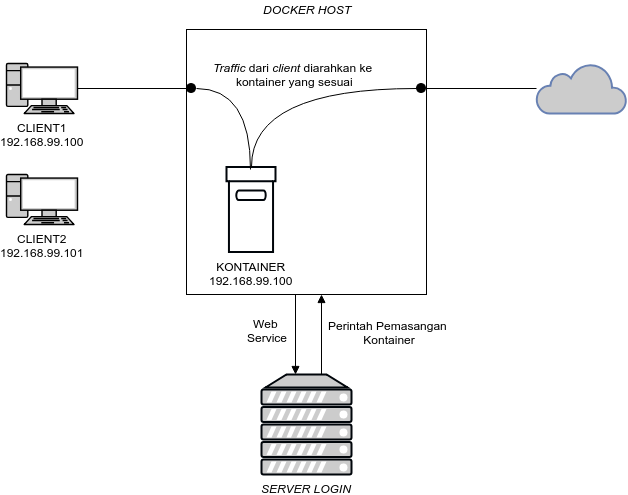
\includegraphics[width=\linewidth]{images/bab4/DIAGRAM3}
	\caption{Arsitektur saat \textit{Traffic} dari \textit{Client} Diarahkan ke Halaman \textit{Login}}
	\label{diagram3}
\end{figure} 